%***********************************************************************
% PLEASE LEAVE THIS PART UNCHANGED
% No problem!
%***********************************************************************

\documentclass[twoside]{report}
\usepackage{iwsm}
\usepackage{graphicx}
\usepackage{amsmath, amssymb}
\usepackage{booktabs}

\begin{document}

%***********************************************************************
% PLEASE INSERT YOUR CONTENT FROM HERE
%***********************************************************************

% Title and running title to be used as left header:
\title{Graphical Assessment of Probabilistic Precipitation Forecasts}
\titlerunning{Graphical Assessment of Probabilistic Forecasts}
%\title{Probabilistic Precipitation Forecasts: Model comparison and Graphical Assessment}
%\titlerunning{Probabilistic Precipitation Forecast Assessment}

% Authors and running list of authors to be used as right header:
\author{Reto Stauffer\inst{1}\inst{2}, Moritz N. Lang\inst{1}, Achim Zeileis\inst{1}}
\authorrunning{Surname 1 et al.}    %% use \authorrunning{Surname 1} if only 1 author
                                    %% use \authorrunning{Surname 1 and Surname2} if two authors
                                    %% use \authorrunning{Surname 1 et al.} if more than two authors

% Institutes of all authors
% Include city and country of each institute, do not include the full address.
\institute{Department of Statistics, Universit\"at Innsbruck, Austria
\and Digital Science Center, Universit\"at Innsbruck, Austria}

% E-mail of presenting author for correspondence
\email{Reto.Stauffer@uibk.ac.at}

% Brief abstract of the paper:
\abstract{
    The demand of accurate and reliable probabilistic predictions
    has seen an strong growth over the past decades and are an essential
    tool for proper risk assessment or strategic planning. In consequence,
    there is an increasing demand on appropriate evaluation methods for
    probabilistic models. Besides proper scoring rules graphical assessment
    methods can be favorable to identify possible model misspecification.

    Distributional regression models are frequently used to provide
    probabilistic predictions, whereof many different flavours and dedicated
    software (packages) have been proposed over the recent years. Thus,
    the calculation of the predictive distribution, probabilities, or quantiles
    is often dependent of the software being used and routines for graphical
    model evaluation are often only available for specific models or distributions
    provided by the corresponding package. An easy generic way of graphically
    evaluate and compare different types of probabilistic models does not yet exist.
    We present a common conceptual framework, a
    flexible object-oriented toolbox for graphical model assessment implemented
    in the \emph{R}\,package \textbf{tompmodels} (\text{https://topmodels.R-forge.R-project.org}).

    The package provides a unified interface to create various visualization
    types including PIT (probability integral tranform) histograms, Q-Q (quantile-quantile)
    plots of (randomized) quantile residuals, wormplots, or rootograms.
    The plots can be rendered in base \emph{R} as well as in \textbf{ggplot2} and provide
    a diversity of options such as adding confidence intervals, sample uncertainties,
    or different scalings.
    To discuss the different types of graphics, how they relate
    to one another and which type of display is particularly useful to bring out
    which type of model deficiencies will be discussed on a case study of
    probabilistic precipitation forecasts for the city of Trieste, Italy.

    %Probabilistic weather forecasts are typically generated by physically
    %based numerical ensemble models providing multiple forecasts with slightly
    %different conditions to depict the forecast uncertainty for a specific situation.
    %Due to the nature of the data and the necessary simplifications these forecasts
    %are not perfect and often show too little uncertainty, especially when compared
    %to sprcific locations.

    %Statistical post-processing is thus commonly used to increase the accuracy
    %and reliability. Distributional regression models have shown to be compatible
    %with other methods proposed over the past decade and allow to not only correct
    %the expectation, but to simultanously adjust the uncertainty.
    %Proper scoring rules, e.g., CPRS or log-scores, are often used to find the
    %best performing model alongside with graphical assessment methods. The latter
    %can be particularely useful to identify possible misspecifications in the
    %model assumption and will be the focus of this contribution.
}

% Keywords (at most 5):
\keywords{Graphical model assessment; Probabilistic prediction; Distributional regression; Precipitation forecasts}

% Produce the title:
\maketitle

%***********************************************************************

% Sections and subsections (do not use lower levels):

\section{Introduction/Background}

Forecasting precipitation has always been one of the essential quantities in
weather forecasting not only for the public, but for many socio-economic areas
like agriculture, power production, but also decison makers with respect risk
assessments. 
The demand of accurate predictions of the expected amount of precipitation has
increased over the past decade where severe precipitation events have increased
in intensity and frequency.

Weather forecasts are typically generated by physically based numerical weather
prediction models. To account for uncertainty, multiple forecasts are created
with slightly modified conditions which build an ensemble (Gneiting et\,al.
2005). This allows to not only retrieve the expected amount of precipitation
but information about the uncertainty of a specific forecast.
To unleash the full potential of these ensemble forecasts, statistical
post-procesing is often used to correct model biases and insufficiencies in
forecast uncertainty. This is especially important when comparing the raw
ensemble forecasts to different spatial scales, e.g., to specific locations.

Probabilistic statistical methods allow to simultanously adjust the
expectation 
...
[Ab ins naechste Meeting]
Over the recent years many probabilistic statistical post-processing methods
have been proposed. .....
allows to imrpove the accuracy and reliability
of these forecasts by comparing historical ensemble forecast and observed
amounts to correct for possible errors.

In the recent past many different
statistical models have been proposed using different distributional assumptions
and learners. For evaluation, proper scoring rules are often used which not
only evaluate the expectation but the full probabilistic distribution of
the forecasts. To identify possible misspecifications in the model
assumption, graphical assessment methods are particularely advantageous
and will be presented in this article.

\section{Data}

Toy data set consisting of X days of accumulated 3-day precipitation
forecasts for station Innsbruck and corresponding observations.

\section{Methodology}

\subsection{Statistical models}

\subsection{Model assessment}

$$
y_i \sim \mathcal{D}(\theta_i | X_i)
$$

Rootogram (Marginal scale):

$$
\text{obs}_j = \sum_{i=1}^n \omega_i I(y_i \in (b_j, b_{j+1}))
$$

$$
\text{exp}_j = \sum_{i=1}^n \omega_i \big[ F(b_{j+1} | \hat{\theta}_i) - F(b_{j} | \hat{\theta}_i) \big],
$$

PIT residuals; CDF evaluated at observation $y_i$ given the
estimated parameters $\hat{\theta}_i$.

$$
u_i = F(y_i | \hat{\theta}_i)
$$


QQ-residuals

$$
\hat{r}_i = \Phi^{-1}\big(F(y_i | \hat{\theta}_i)\big) = \Phi^{-1}(u_i)
$$

for the theoretical quantiles ($z_i$) one typically draws $N$ equidistant
quantiles from the Normal distribution ($\frac{1}{N+1}, ..., \frac{N}{N+1}$),
plotting all pairs $\big((z_{(1)},\hat{r}_{(1)}), ..., (z_{(N)},\hat{r}_{(N)})\big)$

Wormplots: basically the same but detrended

$\big((z_{(1)},\hat{r}_{(1)} - z_{(1)}), ..., (z_{(N)},\hat{r}_{(N)} - z_{(N)})\big)$

\section{Model comparison}

Show plots here, refer to the equations above.

\begin{figure}[!ht]\centering
    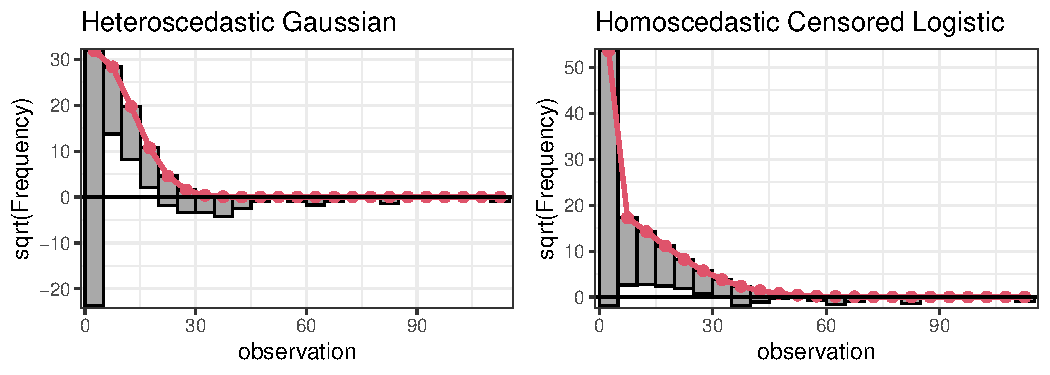
\includegraphics[width=\textwidth]{Stauffer-rootograms}
    \caption{\label{stauffer:fig1} Caption text \textbf{BELOW} the figure.}
\end{figure}

\begin{figure}[!ht]\centering
    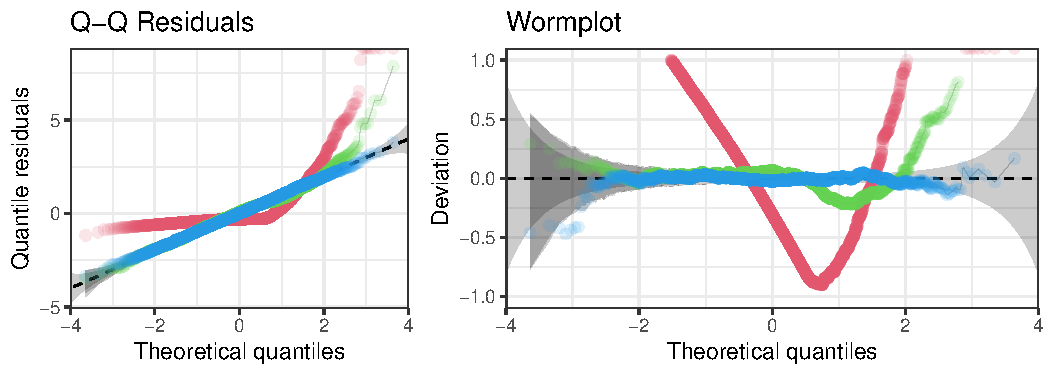
\includegraphics[width=\textwidth]{Stauffer-qqresiduals}
    \caption{\label{stauffer:fig2} Caption text \textbf{BELOW} the figure.}
\end{figure}


%***********************************************************************

% Acknowledgments, if needed:
\acknowledgments{Special Thanks to ... }

%***********************************************************************

% References should be placed in the text in author (year) form.
% The list of references should be placed below IN ALPHABETICAL ORDER.
% (Please follow the format of the examples very tightly).




\references
\begin{description}
% Reliability diagram
\item [Bröcker, J., and Smith, L.A.] (2007).
    Increasing the Reliability of Reliability Diagrams.
    {\it Weather and Forecasting},
    {\bf 22}(3), 651\,--\,61.
% Ensemble forecasting
\item[Gneiting, T, and Raftery, A.E.] (2005).
    Weather Forecasting with Ensemble Methods.
    {\it Science},
    {\bf 310}(5746), 248\,--\,249.
% Proper scoring rules (CRPS)
\item[Gneiting, T, and Raftery, A.E.] (2007).
    Strictly Proper Scoring Rules, Prediction, and Estimation.
    {\it ournal of the American Statistical Association},
    {\bf 102}(477), 359\,--\,78.
% Maximize sharpness subject to calibration
\item[Gneiting, T., Balabdaoui, F., and Raftery, A.E.] (2007).
    Probabilistic Forecasts, Calibration and Sharpness.
    {\it Journal of the Royal Statistical Society: Series B (Methodological)},
    {\bf 69}(2), 243\,--\,68.
% Rootograms (marginal calibration)
\item [Kleiber, C., and Zeileis A.] (2016).
    Visualizing Count Data Regressions Using Rootograms.
    {\it The American Statistician},
    {\bf 70}(3): 296\,--\,303.
% PIT residuals (specifically)
\item [Warton, D.I., Thibaut, L., and Wang, Y.A.] (2017).
    The Pit-Trap---{A} ``Model-Free'' Bootstrap Procedure for Inference About
    Regression Models with Discrete, Multivariate Responses.
    {\it PLOS ONE},
    {\bf 12}(7), 1\,--\,18.
% Reliability diagram
\item [Wilks, D.] (2011).
    {\it Statistical Methods in the Atmospheric Sciences 3rd ed}.
    Academic Press.
\end{description}

\end{document}
